\documentclass[11pt]{article}
\usepackage[a4paper,margin=24mm]{geometry}
\usepackage{fontspec}
\setmainfont{Noto Serif}
\usepackage{microtype}
\usepackage{longtable,booktabs,array}
\usepackage{enumitem}
\usepackage{xurl}
\usepackage{hyperref}
\usepackage{graphicx}
\usepackage{bookmark}
\hypersetup{colorlinks=true,linkcolor=blue,citecolor=blue,urlcolor=blue}
\urlstyle{same}
\setlength{\parindent}{0pt}
\setlength{\parskip}{4pt}
\setlength{\emergencystretch}{3em}
\setcounter{secnumdepth}{2}

\newcommand{\tightlist}{\setlength{\itemsep}{0pt}\setlength{\parskip}{0pt}}


\newcommand{\doctype}{Technical report}

\newcommand{\docversion}{v0.04.003}

\newcommand{\docdate}{30 October 2026}

\newcommand{\versiondoi}{10.5281/zenodo.NNNNNNNN}

\newcommand{\conceptdoi}{10.5281/zenodo.NNNNNNNN}

\newcommand{\docrepo}{github.com/fsantibanezleal/CAOS\_Geophysics}


\newcommand{\headerblock}{%
\begin{center}
\fbox{\parbox{0.94\textwidth}{\small\raggedright
\textbf{\doctype} \quad$\cdot$\quad \docversion, \docdate \quad$\cdot$\quad Licence CC BY 4.0\\[2pt]
CAOS Research open-problems programme \quad$\cdot$\quad product Inverse Earth Studio \quad$\cdot$\quad geophysics\\[2pt]
Version DOI (TODO, draft-only placeholder; not assigned): \texttt{\versiondoi}\\[2pt]
Concept DOI, always latest (TODO, draft-only placeholder; not assigned): \texttt{\conceptdoi}\\[2pt]
Not peer reviewed. Source code, data and computational records: \href{https://github.com/fsantibanezleal/CAOS_Geophysics}{\texttt{\docrepo}}
}}
\end{center}
\vspace{4pt}}

\title{Inverse Earth Studio: a reproducible geophysical workbench for processing, forward modelling, inversion, and scientific review}
\author{Felipe Santib\'a\~nez-Leal}
\date{}
\begin{document}
\maketitle
\headerblock
\begin{abstract}
Geophysical inversion is underdetermined: observations constrain a
subsurface model only through acquisition geometry, a forward operator,
error assumptions, parameterization, prior information, and numerical
optimization. Inverse Earth Studio is an open-source research workbench
connecting data ingestion and processing, forward modelling, inversion,
diagnostics, and interpretation across potential fields,
electromagnetics, electrical methods, and seismology. Its implementation
includes Python pipelines and solvers, bilingual computational
notebooks, provenance-bearing experiments, browser instruments, and a
bounded authenticated-service design.

The method suite spans gravity and magnetic processing and inversion,
magnetotelluric screening and layered-earth inversion,
electrical-resistivity quality control and inversion, waveform
processing and phase picking, travel-time inversion, acoustic
full-waveform inversion, joint inversion, and learned estimators.
Results include both recoveries and failures. For example, a synthetic
gravity case has weighted WRMS 1 while recovered model correlation is
0.283 and centroid depth is about 570 m for a 282 m truth; a
low-velocity FWI case remains unresolved. Clear Lake station cl061 is
retained for tensor quality control and excluded from 1D inversion after
failing the consistency screen. A proposed travel-time residual
refinement shows a small positive result on one fixed synthetic cohort,
which does not establish field transfer or general superiority.

The workbench makes data fit, model recovery, and geological
interpretation separate questions. Synthetic cases carry known truth;
field observations do not. Replayed browser artifacts are distinguished
from online calculations, and notebook execution is distinguished from
scientific validation. The report documents the methods, numerical
assumptions, data provenance, executable results, and limitations; it
does not claim that unresolved scientific or service-acceptance gates
have passed.

\end{abstract}
\clearpage
\section{Scientific motivation}\label{scientific-motivation}

An inverse image can look geologically persuasive even when multiple
models explain the data, the assumed physics are violated, or a withheld
acquisition subset is poorly predicted. This is familiar across
geophysics: potential-field inverses are non-unique; MT dimensionality
and component quality condition whether a 1D interpretation is
defensible; seismic inversion depends on illumination, bandwidth,
starting model, and cycle skipping; and coupled or learned estimates
inherit their structural or training priors. A low objective is evidence
about a specified objective under a specified data model. By itself, it
is not evidence of unique or accurate geology.

The topic sequence draws on the public theoretical-practical geophysical
inversion course by Mantilla. Its notebooks, recordings, images, and raw
data are not redistributed. The source commit was
\texttt{0084021fcc6c1d2f112b144e6e5f0a3d92f20dff} (Mantilla course). The
research survey distinguishes primary sources from implementation
choices and identifies where the methods differ from cited work
(\texttt{docs/research/review.md}). The aim is to connect domain
assumptions, executable calculations, diagnostic evidence, and failure
states within one inspectable project.

The report covers gravity station correction and prism inversion,
aeromagnetic processing, induced-magnetization modelling,
magnetotelluric screening and layered-earth inversion, electrical
resistivity inversion, response-aware waveform processing, first-arrival
tomography, acoustic full-waveform inversion, joint potential-field
inversion, learned seismic-velocity estimation, and earthquake phase
picking. It also evaluates a proposed coverage-conditioned null-space
correction. Method definitions and numerical assumptions are in
\texttt{docs/design/SDD.md}.

\section{Software and evidence
design}\label{software-and-evidence-design}

\subsubsection{2.1 Evidence chain}\label{evidence-chain}

The intended data flow follows the path

\texttt{source\ →\ immutable\ raw\ asset\ →\ validated\ dataset\ →\ processing\ →\ model/survey\ →\ solve\ →\ evaluation\ →\ result/export}.

At each boundary the contracts carry modality, named dimensions and
order, coordinate frame or specified local coordinates, units, geometry,
masks and reasons, uncertainty, parent identities, code/environment
information, and hashes as applicable. Unknown units, datum, signs,
component orientation, rights, or response conventions are reasons to
reject or quarantine an input rather than infer missing facts. Known
truth is attached only to explicitly synthetic cases. Field observations
may be screened and processed, but a synthetic constructor is never
substituted for missing field provenance or truth.

The application separates three execution contexts. Visitors can inspect
public material and use only those browser calculations whose
client-side behavior has been validated. Authenticated project workflows
are designed to isolate upload, ownership, and bounded worker execution
on the single canonical ML VPS origin. Larger training, extensive FWI,
and full bake workflows remain local CPU/GPU pipelines. A static or
browser replay of a saved artifact is not represented as an online
inverse solve. The specified deployment uses one bounded ML VPS service.
Its capacity and numerical job behavior have not been measured on the
live host.

\subsubsection{2.2 Reproducible software
artifacts}\label{reproducible-software-artifacts}

The software contains a Python data pipeline and solver implementations,
generated and source-controlled scientific outputs, JSON contracts and
validation outputs, frontend TypeScript/React instruments, and
computational notebooks in English and Spanish. The user-facing browser
is intended to display computed arrays and explicit physical axes, not
to invent a second approximate result for animation. Physical result
records distinguish observations, predictions, signed residuals, model
values, objective terms, coverage and uncertainty diagnostics, stopping
state, and provenance. Display interpolation or color mapping is a
rendering operation and must not be mistaken for increased model
resolution.

Notebooks are part of the research material, not merely screenshots.
Their lessons explain assumptions, execute the named calculations, show
numerical outputs, compare with independent identities or baselines when
available, and retain unresolved results. The bilingual content was
corrected where translations, counts, or numerical interpretations
differed. Execution and translation checks establish neither field
validity nor educational efficacy.

\section{Data and experimental scope}\label{data-and-experimental-scope}

\subsubsection{3.1 Authored synthetic
experiments}\label{authored-synthetic-experiments}

The original canonical suite uses independently constructed geological
geometries instead of repeating one centered anomaly. Its earlier 0.04
report describes 20 distinct cases and six controlled conditions per
case (120 experiments, 348 method results). The conditions vary
contrast, noise, acquisition, coverage, or regularization according to
the physical family; they are not interchangeable perturbations and are
not samples from a geological population. Later repository work adds
separate survey, uploaded-data, learning, and source-screening
experiments. Therefore the older 120-experiment suite is a defined
artifact family, not a count of every experiment now present in the
repository.

Synthetic constructors provide known truth for controlled tests of
forward physics and conditional inversion behavior. They do not encode
the full complexity of field geology. Noise perturbations at fixed
mesh/prior/tradeoff measure conditional estimator repeatability, not
posterior uncertainty. A held-out line, shot, family, or acquisition
tests only the specified split and comparator. Repeated numerical trials
from one generator do not establish field performance.

\subsubsection{3.2 External data and
eligibility}\label{external-data-and-eligibility}

Two SimPEG tutorial archives are independently pinned and locally
preprocessed as ingestion examples. The source documentation states that
their derived observation tables are not redistributed while upstream
redistribution rights remain unresolved. They are not field validation.
The measured Clear Lake EDI station cl061 is hash-pinned and cited to
the USGS and EarthScope data releases
\cite{usgsClearLake,earthscopeClearLake}. Its impedance tensor fails the
required 1D consistency screen; it remains a QC-only dataset, and no
layered inversion or geological result is claimed.

Other data paths include provider-linked or rights-restricted data. For
example, the Slagdump ERT raw asset is absent locally under its
provider-link-only status; focused notebook checks consequently skip
tests that require those bytes. The Koenigsee travel-time lesson is an
authored synthetic method control and does not establish execution on
the provider-linked case. The M13 STEAD excerpts \cite{mousavi2019} and
associated project-trained checkpoint have a scoped redistribution
decision with attribution; that decision does not generalize to other
data or establish model accuracy. Rights, data custody, field
eligibility, numerical correctness, and scientific validation remain
separate decisions.

\section{Methods}\label{methods}

The method identifiers below follow \texttt{docs/design/SDD.md}. Each
entry names an implementation and its tests; this does not imply
validated use for every input or a complete end-to-end workflow.

\begin{center}\small
\begin{longtable}{@{}p{0.12\textwidth}p{0.40\textwidth}p{0.41\textwidth}@{}}
\toprule
Method & Executable purpose & Principal limitations \\
\midrule
\endfirsthead
\toprule
Method & Executable purpose & Principal limitations \\
\midrule
\endhead
Gravity corrections and transforms & Gravity station corrections, datum and uncertainty lineage, and transforms with safeguards against duplicate corrections. & Field eligibility still depends on exact source, datum, instrument, and uncertainty lineage. A local adapter pass does not validate arbitrary field tables. \\
Weighted 3D gravity prism inversion & Weighted 3D gravity prism forward/inverse calculations, including a bounded L2 survey inversion and comparison with independent prism physics. & Non-uniqueness persists; a good data fit or a visually compact body does not identify geology. Full-survey and field performance remain untested. \\
Aeromagnetic processing and continuation & Aeromagnetic line/tie-line/height checks, blocked line holdout, support-aware gridding, and physically supported upward continuation. & Authored survey controls do not establish broad provider-data validation or field magnetic inversion. \\
Induced-magnetization prism modelling & Induced-magnetization prism forward modelling and physical objective/derivative construction, checked against Choclo. & A full nonzero survey inverse with held-out evaluation is not included in the available evidence. Remanence violates the induced-direction assumption. \\
EDI quality and dimensionality screening & MT EDI component, variance, rotation, tipper, and dimensionality screening. & A tensor record is not automatically eligible for a 1D inverse. cl061 remains QC-only. \\
Layered-earth impedance inversion & Layered-earth complex-impedance response and bounded 1D inversion, with cross-checks against MTpy and browser/local analytic cases. & Known layer thickness and isotropic 1D assumptions constrain the synthetic inverse. The cl061 field screen fails. \\
Two-dimensional electrical resistivity inversion & 2D ERT processing/inversion with electrode geometry, topography, reciprocal/QC logic, blocked holdout, and explicit failed-inverse states. & Rights-restricted raw data are not fabricated or represented as executed; independent comparison and some field paths remain open. \\
Response-aware waveform processing & MiniSEED/StationXML waveform handling, response-aware filtering, STA/LTA or matched-arrival picks. & Response epochs, units, gaps, and channel orientation are strict eligibility conditions. STA/LTA picks are not universal truth labels. \\
First-arrival travel-time inversion & First-arrival travel-time inversion with explicit source/receiver geometry, bounded velocity, ray coverage, and held-out-shot comparison against a baseline. & The executed teaching control is synthetic and uses a straight-ray/Dijkstra model; the synthetic control does not represent provider-linked field data. \\
Acoustic full-waveform inversion & Acoustic constant-density FWI with Deepwave, bounded velocity updates, full-band and frequency-continuation schedules, active/withheld receiver diagnostics, and saved optimizer states. & Non-convexity, cycle skipping, limited illumination, inverse crime from using the same forward engine, and acoustic-only physics remain material limitations. Some cases improve model RMSE but fail the specified noise-consistency criterion. \\
Joint potential-field inversion & Joint potential-field inversion comparing uncoupled fits, spatial cross-gradient coupling, and an explicit Gaussian-mixture petrophysical prior. & The project Gaussian-mixture-prior implementation is not the SimPEG PGI optimizer. Coupling can trade one property against another; one calibration matrix does not establish general performance. \\
Learned seismic-velocity estimation & A learned seismic-velocity inversion trained on disjoint procedural families and compared with a same-input weighted L2 solve and independent quadrature forward operator. & The frozen joint family/acquisition holdout fails both prespecified ratios; training success does not override the held-out result. \\
PhaseNet-family phase picking & PhaseNet-family P/S inference \cite{zhu2019}, matched STA/LTA comparison, and local browser ONNX inference with explicit preprocessing and abstention rules. & Curated browser parity is runtime consistency, not accuracy. Population metrics come from the separate locked test cohort and analyst references, not geological truth. \\
Coverage-conditioned null-space velocity correction & Geometry-normalized backprojection of travel-time residuals, divided by path length and cell coverage, supplied with a coverage channel to a bounded residual CNN. & It is a falsifiable refinement proposal. The initial checkpoint 3.1 failed the joint-shift comparison; the later null-space-constrained variant gives a narrow synthetic improvement but does not change the M12 checkpoint result or establish field transfer. \\
\bottomrule
\end{longtable}
\end{center}

\subsubsection{4.1 Potential-field
inverses}\label{potential-field-inverses}

The gravity and magnetic experiments use SimPEG rectangular-prism
sensitivity operators \cite{cockett2015,heagy2017}, explicit survey
geometry, uncertainty-weighted data residuals, and spatial
regularization. The canonical potential-field setup uses a 10,752-cell
mesh and 256 surface observations
(\texttt{docs/research/scientific-implementation.md}). L2 and
smoothed-L1 IRLS solutions are distinct estimators, not interchangeable
render styles. Magnetic cases include scalar induced assumptions and
vector magnetization so that remanence can be exposed as model
misspecification. Choclo prism values \cite{choclo} provide an
independent physical check for sign and scale in specified comparisons.
Sensitivity and conditional noise ensembles are not interpreted as
calibrated geological posterior intervals.

The current result table includes a gravity deep-body example for which
weighted WRMS is 1, while model correlation is only 0.283 and recovered
centroid depth is approximately 570 m versus a synthetic truth near 282
m. This is not a paradox: the inverse fits the observations at the
chosen noise scale while regularization and limited information admit a
different model. The structure is unresolved despite the weighted data
fit.

\begin{figure}[!t]
\centering
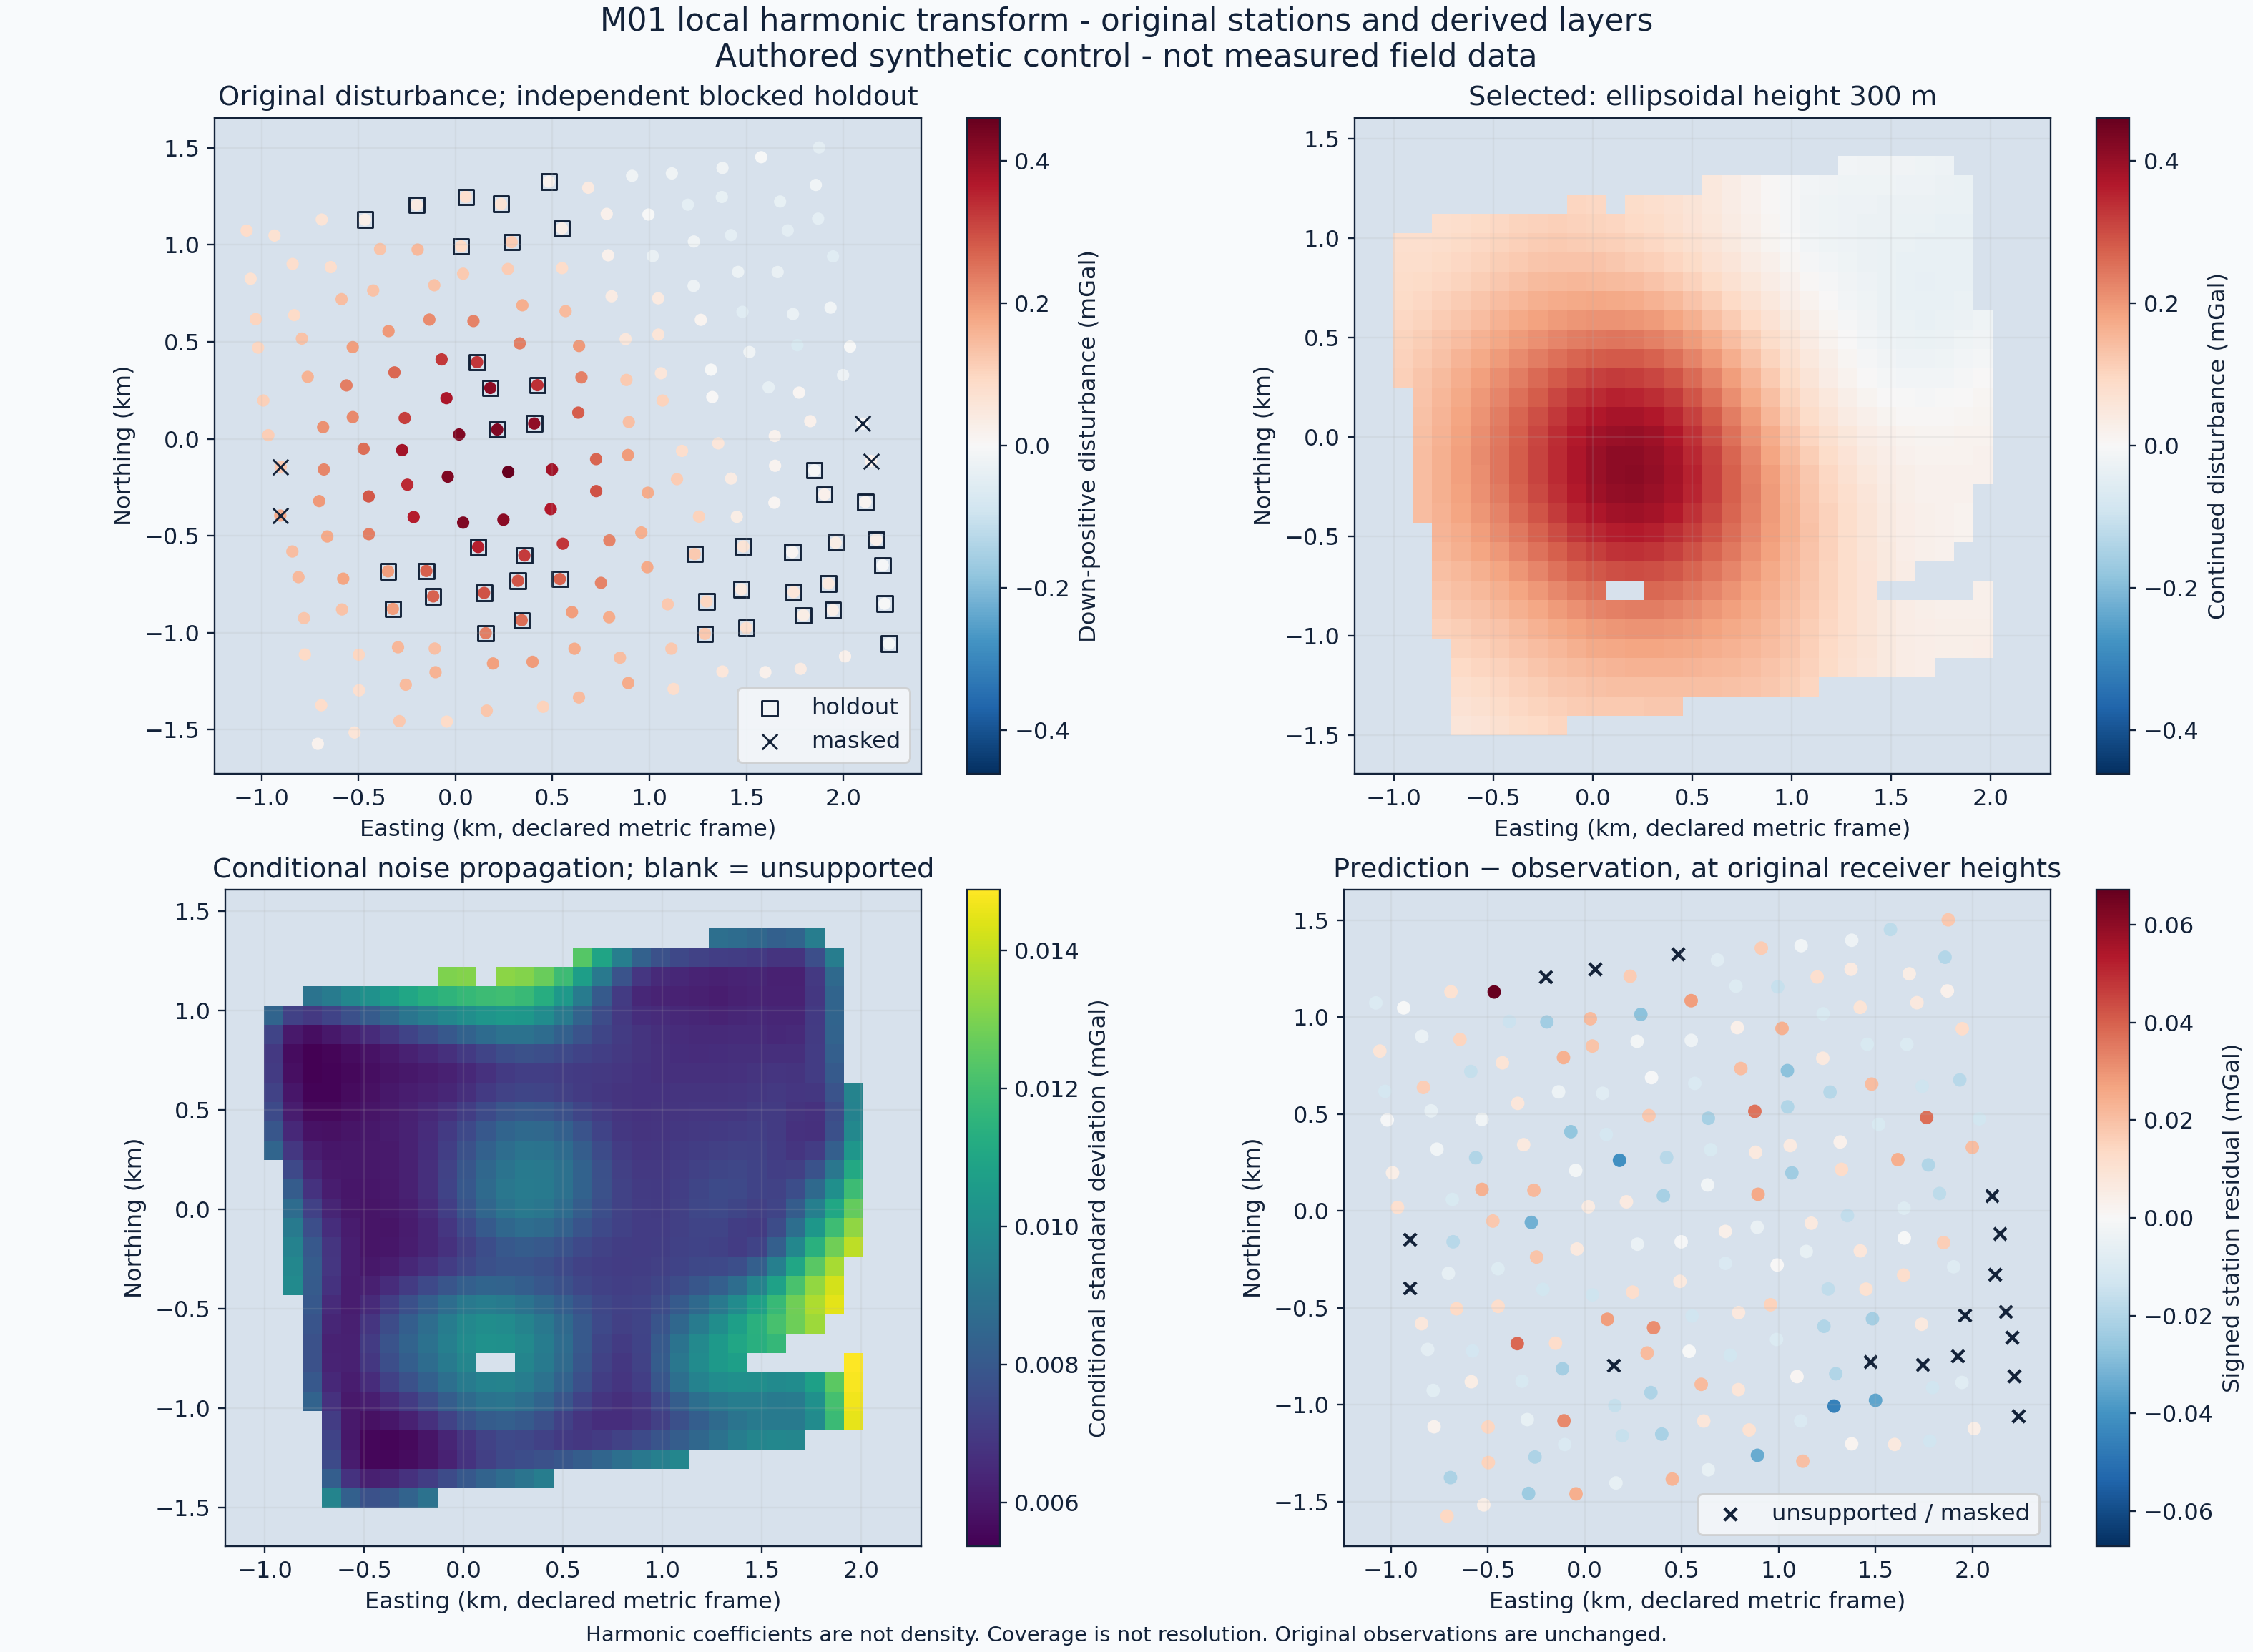
\includegraphics[width=0.95\linewidth,height=\textheight,keepaspectratio,alt={M01 authored synthetic control. Upper left: original station disturbance and blocked holdout or masked locations. Upper right: harmonic continuation to 300 m. Lower left: propagated conditional noise standard deviation, with blank cells unsupported. Lower right: signed prediction residuals at original receiver locations. The figure is synthetic and does not represent field measurements.}]{figures/m01-height-continuation.png}
\caption{M01 authored synthetic control. Upper left: original station
disturbance and blocked holdout or masked locations. Upper right:
harmonic continuation to 300 m. Lower left: propagated conditional noise
standard deviation, with blank cells unsupported. Lower right: signed
prediction residuals at original receiver locations. The figure is
synthetic and does not represent field measurements.}
\end{figure}

\subsubsection{4.2 MT, ERT, and waveform
processing}\label{mt-ert-and-waveform-processing}

The MT response is calculated through the complex impedance recursion
for isotropic layers; differentiable physics-guided inversion is a
related approach \cite{goyes2025}. EDI ingestion is a transfer-function
workflow and preserves conventions, units, rotations, masks, and stated
variances; EDI is not treated as raw time-series data. Multiple
optimizers (bounded least squares, Adam, and a small per-sounding neural
parameterization) address matched objectives in synthetic fixtures. A
neural architecture related conceptually to physics-guided inversion
\cite{goyes2025} is not asserted to reproduce the cited paper's
architecture or published results.

ERT workflows validate electrode/ABMN structure, QC and topographic
factors before inversion, following established 2D methods such as
PyGIMLi \cite{pygimli}. The numerical examples distinguish authored
controls from absent or restricted field assets and retain failed
inversions. Seismic preprocessing distinguishes instrument counts,
response-corrected units, filters, gaps, and sample windows. STA/LTA
picking and M13 learned inference consume explicitly specified traces;
analyst picks are reference annotations, not subsurface truth.

\subsubsection{4.3 Travel-time tomography, FWI, and joint
inversion}\label{travel-time-tomography-fwi-and-joint-inversion}

Travel-time inversion uses specified ray geometry and a
training/withheld partition. Its velocity maps are interpreted together
with ray support; unsupported cells do not receive equivalent evidential
status. The M09 bilingual lesson calls the product inverse core on an
authored refracting two-layer survey and compares complete withheld
shots with a training-only homogeneous baseline. This is a bounded
synthetic calculation.

The FWI implementation uses constant-density acoustic propagation
\cite{virieux2009,deepwave}, a fixed acquisition family, bounded
velocity, a data-derived coarse background, and matched update budgets
for full-band and frequency-continuation schedules. Active and withheld
receiver WRMS accompany model RMSE. A lower model RMSE can coexist with
residuals above the specified noise level. The four-case computation
includes a layered reflection, a fault, a salt/cycle-skipping negative
control, and a low-velocity channel. Its case-level results are not
generalized to field-scale FWI or elastic/attenuating physics.

Joint inversion compares uncoupled and coupled estimates against the
same observations and independent baselines. Cross-gradient coupling
promotes structural similarity, while a Gaussian-mixture prior adds a
distinct petrophysical assumption \cite{simpegJoint,astic2020}. These
mechanisms are reported separately. In the shared synthetic case,
cross-gradient slightly improves susceptibility RMSE while worsening
density RMSE relative to the optimized uncoupled solution; the
mixture-prior method slightly improves density RMSE while slightly
worsening susceptibility. Neither is a joint two-property recovery gain.
In a deliberately conflicting case, the negative control rejects a
general claim that structural or petrophysical coupling must help.

\subsubsection{4.4 Learned methods and the beyond-established
experiment}\label{learned-methods-and-the-beyond-established-experiment}

The original gravity CNN predicts column density rather than a
depth-resolved volume, reflecting the non-identifiability of depth from
one potential-field map. Learned inverse benchmarks also show
sensitivity to the sampled geological families \cite{openfwi}. Its
comparison with a spatial L2 baseline uses identical seeded noisy
observations and a shared column target. The autoencoder's threshold is
selected on a separate calibration set and tested on withheld
geometries; its measured failure to detect the withheld family is
retained. These models are compact baselines and have not been compared
with a broader set of published inverse methods.

M12 predicts seismic velocity from travel-time data and is evaluated by
family/acquisition-disjoint cohorts. The 2026-10-28 M12 computation used
160 joint family/acquisition holdouts with learned/weighted-L2 velocity
RMSE 536.99/95.62 m/s (ratio 5.616) and independent-oracle travel-time
RMSE 28.61/2.34 ms (ratio 12.231; source:
\texttt{docs/validation/m12-checkpoint-notebook-2026-10-28.md}). Both
pre-specified comparison criteria fail. A separate checkpoint 3.1 run
also fails its specified joint-shift comparisons. The separate
null-space-constrained residual study reports velocity RMSE ratio 0.9701
(paired case-bootstrap interval 0.9661--0.9737) and independent
travel-time RMSE ratio 0.9967 (0.9950--0.9983); the aggregate ratios
improve in all four fixed held-out cohorts. The v1.1 scorer used an
infinite threshold, so the saved exceedance counts are not a valid
threshold assessment and are not interpreted here. The paired intervals
resample case IDs and compute the ratio of mean per-case RMSEs over
20,000 PCG64 draws (seed 6122026); the exact calculation is retained in
\texttt{docs/validation/m12-nullspace-v1\_1-bootstrap-2026-10-30.json}.
These intervals quantify variation within the fixed synthetic cohorts,
not natural-geology uncertainty. The result is specific to that protocol
and cohort. It does not change the failing M12 checkpoint result,
establish geological recovery, or demonstrate field transfer.

The proposed coverage-conditioned correction asks whether a
dimensionally consistent, coverage-conditioned learned residual improves
on a matched weighted L2 inverse under geometry shifts. The proposal is
falsifiable because model and independent forward-data ratios are frozen
and both must be below one for an advantage claim. The differing
outcomes show why protocol and checkpoint identity must accompany each
comparison.

\section{Selected results and
interpretation}\label{selected-results-and-interpretation}

\subsubsection{5.1 Reference-condition
outcomes}\label{reference-condition-outcomes}

The reference-condition summary lists 122 recovered, 184 unresolved, 6
failed, and 36 negative-control method results (source:
\texttt{docs/validation/results.md}). These are case-specific outcomes.
They must not be summed into an overall accuracy or treated as success
probabilities because the cases, units, target variables, and criteria
differ. Failure and unresolved outcomes are first-class evidence in this
project.

\subsubsection{5.2 FWI case matrix}\label{fwi-case-matrix}

The bilingual case-matrix lesson reads four hash-verified full-run
arrays
(\texttt{notebooks/en/06-seismology/05-m10-fwi-case-matrix.ipynb};
Spanish counterpart). Layered reflection and fault are labeled recovered
under the case-specific criteria; salt remains a cycle-skipping negative
control; and the low-velocity channel remains unresolved. For the
channel, model RMSE improves relative to the starting model (ratio 0.521
for the continuation result), but fitted/withheld WRMS are 2.071/2.213
against the specified unit noise scale. This contrast shows why
improvement from a starting model is not sufficient. The notebook
re-analyzes saved output rather than re-solving FWI, and an independent
propagator comparison is needed to test sensitivity to using the same
forward engine.

\subsubsection{5.3 EDI screening and phase
picker}\label{edi-screening-and-phase-picker}

The observed cl061 EDI tensor is screened against necessary 1D
consistency conditions and fails them. It remains QC-only. It provides
no 1D resistivity model for cl061 and makes no geological interpretation
from that station. For M13, the 2026-10-27 local browser parity
computation reports all 23 valid selected display traces matching CPU
ONNX Runtime: maximum absolute probability difference 5.0664×10⁻⁶, no
P/S peak displacement, and matching accepted/abstained picks within one
sample. A twenty-fourth selected trace is QC-rejected and never
inferred. The separate locked 6,000-trace benchmark, not this curated
23-trace subset, is the population-level performance record. Even that
benchmark compares predictions with analyst annotations and should not
be described as geological truth.

\subsubsection{5.4 Nullspace-constrained learned
refinement}\label{nullspace-constrained-learned-refinement}

The null-space-constrained computation uses a fixed cohort and reports
velocity and independent forward-data ratios with paired case-bootstrap
intervals. Each replicate resamples case IDs and computes the ratio of
mean per-case RMSEs; 20,000 PCG64 draws use seed 6122026. The exact
intervals, method protocol and receipt hash are archived with the
computational outputs. For the joint-OOD cohort, velocity RMSE ratio is
0.9701 with interval 0.9661--0.9737; independent travel-time RMSE ratio
is 0.9967 with interval 0.9950--0.9983. The metrics show a small
synthetic aggregate difference and do not establish a practical gain
across field settings. Field robustness, performance under realistic
source/model error, and reproduction by an external group have not been
evaluated. The v1 computation was invalidated by a dimensional feature
error; the checkpoint 3.1 computation remains a failed comparison.

\section{Educational and visualization
design}\label{educational-and-visualization-design}

The bilingual notebook sequence covers inverse-problem foundations,
gravity, magnetics, MT, ERT, seismology, joint inversion, and learning.
Lessons include progressively deeper content: from units and forward
physics to actual solver calls, held-out evaluation, sensitivity
analyses, independent oracles, and negative controls. The notebooks are
intended as research and teaching materials, but no educational efficacy
study has been performed. The source course is cited as inspiration; its
instructional materials are not copied into the product.

Scientific visualization is organized around the method's actual state
variables. Potential-field scenes show geometry, cells, survey
observations, cuts, and physical property scales; MT views show layer
structure and frequency response; seismic instruments relate wavefields,
receiver gathers, and inversion state; learned methods show their actual
target arrays and comparison metrics. Camera rotation changes viewpoint,
not physics. Time cursors and optimizer-state replay address different
quantities and are labeled accordingly. A rendered state alone is not
evidence of uniqueness, resolution, or uncertainty.

The scientific views expose physical geometry, survey support, and
computed states. Their effect on interpretation has not been measured in
a user study, and browser performance has not been characterized across
devices, routes, languages, and themes.

\section{Computational
reproducibility}\label{computational-reproducibility}

All 60 bilingual notebooks were run from top to bottom in fresh kernels
on 30 October 2026. The computation comprised 57 unchanged notebooks and
three refreshed notebooks; none ended with an execution error. Focused
fresh-kernel replays of the refreshed examples then passed. The complete
replay used \texttt{scripts/run\_notebooks.py\ -\/-check} with external
scratch storage. Notebook sources are under \texttt{notebooks/en/} and
\texttt{notebooks/es/}.

Numerical outcomes are tied to their method-specific computation and
date. The FWI case matrix reads hash-verified outputs and does not rerun
the expensive inverse; its source is
\texttt{notebooks/en/06-seismology/05-m10-fwi-case-matrix.ipynb} and the
Spanish counterpart. The M12 notebook computation dated 28 October and
browser-parity computation dated 27 October are documented computations
in \texttt{docs/validation/m12-checkpoint-notebook-2026-10-28.md} and
\texttt{docs/validation/m13-browser-population-parity-2026-10-27.md}.
The null-space refinement results and cohort definitions are in
\texttt{docs/design/features/m12-velocity-validation/nullspace-v1\_1-protocol.md}.
Reference-condition metrics are in \texttt{docs/validation/results.md}.
Method equations, implementation details, and primary-source mapping are
in \texttt{docs/research/scientific-implementation.md},
\texttt{docs/research/review.md}, and \texttt{docs/design/SDD.md}.

Notebook replay verifies execution for the recorded source and
environment; it is not an independent physical oracle. Scientific
replication requires using the method-specific data, environment, split,
seed, operator, and comparison criteria together. A lesson that reads an
archived computation must not be described as having recomputed that
solve.

\section{Limitations and open research
questions}\label{limitations-and-open-research-questions}

\begin{enumerate}
\def\labelenumi{\arabic{enumi}.}
\tightlist
\item
  \textbf{Field validation and eligibility.} Most quantitative recovery
  results are synthetic. Provider data with incomplete datum,
  uncertainty, rights, or provenance remain unresolved or ineligible.
  cl061 is a QC failure for 1D inversion, not a field inverse.
\item
  \textbf{Non-uniqueness and uncertainty.} Conditional ensembles do not
  sample geological posterior uncertainty. Potential-field structure
  remains prior- and parameterization-dependent. Coverage and
  sensitivity do not by themselves yield calibrated resolution.
\item
  \textbf{FWI scope.} The experiments use bounded acoustic physics and
  fixed synthetic acquisition families. Source uncertainty, realistic
  correlated noise, anisotropy, elasticity, attenuation, broader
  cycle-skipping regimes, and an independent propagator remain necessary
  research directions.
\item
  \textbf{Joint inversion.} Cross-gradient and mixture-prior outcomes
  depend on their scale, prior, and structural compatibility. The
  limited calibration matrix does not establish general superiority over
  optimized single-modality estimates.
\item
  \textbf{Machine learning.} The M12 learned-velocity calculation fails
  its pre-specified joint-shift comparison. The positive null-space
  variant is narrow synthetic evidence and needs external reproduction
  and broader cohorts. The phase-picker's 23-trace parity set is not an
  accuracy cohort; the separate 6,000-trace benchmark uses analyst
  annotations whose uncertainty limits the interpretation of timing
  scores.
\item
  \textbf{Data and reproducibility.} Some numerical tests require
  retained external inputs, including joint-inversion matrices and
  magnetic controls. Missing inputs are not replaced with synthetic
  stand-ins. Rights-limited source files are not copied merely to make a
  computation executable.
\item
  \textbf{Service capacity.} Local solver tests, builds, and browser
  parity do not establish worker admission, VPS capacity, cancellation,
  or recovery. Replacement-service capacity and operational behavior
  remain unmeasured.
\item
  \textbf{Educational effectiveness.} A bilingual executable notebook
  collection is a learning resource, but no controlled study establishes
  learning outcomes or comparative pedagogical effectiveness.
\end{enumerate}

Useful next studies include preregistered geological-family and
acquisition/noise ensembles; external reproduction of the null-space
correction result; calibration under forward-model and geological
uncertainty; independent FWI propagation; licensed field inversions with
source/datum/error review; and user studies of whether linking
assumptions, predictions, residuals, and uncertainty improves
interpretation.

\section{Conclusions}\label{conclusions}

Inverse Earth Studio combines source-linked geophysical processing and
inverse methods with explicit assumptions, independent physical checks
where available, and preserved negative evidence. Its central examples
show that data fit, model recovery, transfer, and visual plausibility
are different questions. The workbench includes synthetic and bounded
real-data screening calculations, bilingual executable notebooks, and
computational paths across multiple physical methods.

These computations do not establish field validity or generality across
geological settings. Several method-specific comparisons, end-to-end
user-supplied-data workflows, actual-host measurements, independent
solver comparisons, and user-facing visual evaluations remain to be
completed. The learned travel-time refinement has a narrowly positive
synthetic result alongside failed variants and a separate M12 failure;
no general learned advantage follows. The work provides a reproducible
software and experimental framework that makes assumptions and
counterexamples inspectable. Algorithmic novelty and publication
priority are not established.

\section{Data and code availability}\label{data-and-code-availability}

Source code is available at
\texttt{https://github.com/fsantibanezleal/CAOS\_Geophysics}. Scientific
methods, notebooks, test data, computational records, and source-rights
decisions are linked above and organized in \texttt{data/},
\texttt{data-pipeline/}, \texttt{docs/}, \texttt{notebooks/},
\texttt{tests/}, and \texttt{models/}. Some external raw observations
are absent because redistribution rights or field eligibility remain
unresolved. The intended application origin is
\texttt{https://geophysics.ml.fasl-work.com/}. Local computations do not
establish replacement-service capacity.

\section{Acknowledgements}\label{acknowledgements}

The work uses and cites open scientific software and public geophysical
data sources listed below and in the repository's research review. No
endorsement by the cited software or dataset authors is implied.


\begin{thebibliography}{99}
\bibitem{cockett2015} R. Cockett, L. J. Heagy, A. Pidlisecky, and D. W. Oldenburg, ``SimPEG: An open source framework for simulation and gradient based parameter estimation in geophysical applications,'' \emph{Computers \& Geosciences}, vol. 85, pp. 142--154, 2015. \href{https://doi.org/10.1016/j.cageo.2015.09.015}{doi:10.1016/j.cageo.2015.09.015}.
\bibitem{heagy2017} L. J. Heagy, R. Cockett, S. Kang, G. K. Rosenkjaer, and D. W. Oldenburg, ``A framework for simulation and inversion in electromagnetics,'' \emph{Computers \& Geosciences}, vol. 107, pp. 1--19, 2017. \href{https://doi.org/10.1016/j.cageo.2017.06.018}{doi:10.1016/j.cageo.2017.06.018}.
\bibitem{goyes2025} P. Goyes-Pe\~nafiel et al., ``Physically guided deep unsupervised inversion for 1D magnetotelluric models,'' \emph{IEEE Geoscience and Remote Sensing Letters}, 2025. \href{https://doi.org/10.1109/LGRS.2025.3528767}{doi:10.1109/LGRS.2025.3528767}.
\bibitem{virieux2009} J. Virieux and S. Operto, ``An overview of full-waveform inversion in exploration geophysics,'' \emph{Geophysics}, vol. 74, no. 6, pp. WCC1--WCC26, 2009. \href{https://doi.org/10.1190/1.3238367}{doi:10.1190/1.3238367}.
\bibitem{deepwave} Deepwave, ``Full waveform inversion example and documentation.'' \url{https://ausargeo.com/deepwave/example_fwi}.
\bibitem{mousavi2019} S. M. Mousavi, Y. Sheng, W. Zhu, and G. C. Beroza, ``STanford EArthquake Dataset (STEAD): A global data set of seismic signals for AI,'' \emph{IEEE Access}, vol. 7, pp. 179464--179476, 2019. \href{https://doi.org/10.1109/ACCESS.2019.2947848}{doi:10.1109/ACCESS.2019.2947848}.
\bibitem{zhu2019} W. Zhu and G. C. Beroza, ``PhaseNet: A deep-neural-network-based seismic arrival-time picking method,'' \emph{Geophysical Journal International}, vol. 216, no. 1, pp. 261--273, 2019. \href{https://doi.org/10.1093/gji/ggy423}{doi:10.1093/gji/ggy423}.
\bibitem{choclo} Fatiando a Terra, \emph{Choclo: geophysical forward modelling with equivalent sources}. \url{https://www.fatiando.org/choclo/latest/overview.html}.
\bibitem{pygimli} PyGIMLi, \emph{Inversion guide and ERT examples}. \url{https://www.pygimli.org/user-guide/inversion/}.
\bibitem{simpegJoint} SimPEG, \emph{Joint inversion with cross-gradient regularization}. \url{https://docs.simpeg.xyz/latest/content/user-guide/tutorials/13_joint_inversion/plot_inv_3_cross_gradient_pf.html}.
\bibitem{astic2020} T. Astic et al., ``Joint inversion of geophysical data with a petrophysical prior.'' \url{https://arxiv.org/abs/2002.09515}.
\bibitem{openfwi} W. Lu et al., ``OpenFWI: Large-scale multi-structural benchmark datasets for seismic full waveform inversion.'' \url{https://github.com/lanl/OpenFWI}.
\bibitem{course} A. G. Mantilla, \emph{Curso te\'orico-pr\'actico sobre inversi\'on geof\'isica en Python}, source commit \texttt{0084021fcc6c1d2f112b144e6e5f0a3d92f20dff}. \url{https://github.com/Anagabrielamantilla/inversion-geofisica-python}.
\bibitem{mtpy} MTpy v2, \emph{Magnetotelluric data and EDI documentation}. \url{https://mtpy-v2.readthedocs.io/en/stable/index.html}.
\bibitem{usgsClearLake} U.S. Geological Survey, \emph{Magnetotelluric data, Clear Lake region, northern California}. \href{https://doi.org/10.5066/P14KAQ3M}{doi:10.5066/P14KAQ3M}.
\bibitem{earthscopeClearLake} EarthScope, \emph{EMTF transfer-function collection: Clear Lake}. \href{https://doi.org/10.17611/DP/EMTF/GMEG/Clearlake}{doi:10.17611/DP/EMTF/GMEG/Clearlake}.
\end{thebibliography}

\end{document}
